

\documentclass{article}
\usepackage{amsmath, amssymb, graphicx, subcaption, tabularx}  % For \mathbb command


    \title{Practicas MC}
    \date{\today}
    \author{Juan Luis Torres Ramos}

    \begin{document}
        
        % 
        % Portada
        % \pagenumbering{gobble}
        % \maketitle
        % \newpage
        % \pagenumbering{arabic}

        \begin{titlepage}
            \centering
            {
\includegraphics[width=1\textwidth]{./Imagenes/logo_universidad_de_granada.png}\par}
            \vspace{1cm}
            {\scshape\Large Escuela Tecnica Superior de Ingenieria Informatica y Telecomunicaciones \par}
            \vspace{2.5cm}
            {\scshape\Huge Examen Modelos de Computación \par}
            \vspace{1cm}
            {\itshape\Large  Grupo B3 \par} 
            \vfill
            {\Large Juan Luis Torres Ramos \par}
            \vspace{0.5cm}
            {\large 24 Octubre 2023 \par}
        \end{titlepage}


        % 
        % Ejercicio 1
        %

        \section*{Ejercicio 1}
            \textbf{Obtener un modelo de calculo para $L = \{ U \mid U \in \{a, b\}^{\pm} \text{ y } N_a(U) = N_b(U) \}$.}
            
            \vspace{\baselineskip} % paso linea
            Queremos encontrar un modelo de cálculo para este lenguaje. Para ello intentaremos estudiar todos los casos posibles.
            \vspace{\baselineskip} % paso linea

            Para programar la gramática que genera este lenguaje, primero observamos que busca cadenas con el mismo número de $b$'s que de $a$'s. 
            Intentaremos encontrar una gramática libre de contexto. Al aplicar el lema del bombeo, nos dice que el lenguaje no es regular.
            \vspace{\baselineskip} % paso linea

            Comenzamos con la producción inicial $S$ que genera $a$ y algo más, es decir, $S \rightarrow aX$, donde $X$ es una variable que determinaremos. 
            Esta producción debe garantizar que no se viole la condición $N_a(b) = N_b(b)$. Esto nos lleva a la producción $S \rightarrow aB$, 
            con $B \rightarrow b$, esta ultima produccion simepre va a haber una $b$ de más.
            \vspace{\baselineskip} % paso linea

            De igual manera, razonamos en la dirección opuesta 
            y obtenemos $S \rightarrow bA$ con $A \rightarrow a$. 
            Hasta este punto, hemos definido cuatro producciones.
            \vspace{\baselineskip} % paso linea

            Ahora, estudiamos el caso de la producción $S \rightarrow aB \rightarrow abX$. Este caso nos centraremos cuando $B \rightarrow bX$,como queremos mantener la 
            condicion de B (tener una $b$ de más). Observamos que $B \rightarrow bS$ cumple con la condicion ($S$ genera una a y una b para este caso). 
            De manera análoga, obtenemos $A \rightarrow aS$ para el caso contrario.
            \vspace{\baselineskip} % paso linea

            Estudiamos el caso $B \rightarrow aX$. 
            Necesitamos una $b$ adicional para cumplir la condición de $B$ , 
            así que definimos $B \rightarrow aBB$, asegurando que la primera 
            $B$ compense una $a$ y luego llamando nuevamente para tener un $B$ 
            adicional. De manera inversa, obtenemos $A \rightarrow bAA$.
            \vspace{\baselineskip} % paso linea

            La gramática libre de contexto resultante es:
            \vspace{\baselineskip} % paso linea
            $G = (V, T, P, S)$ donde $V = \{S, A, B\}$, $T = \{a, b\}$, y $P$ es el conjunto de producciones:
            \vspace{\baselineskip} % paso linea

            \begin{tabularx}{\textwidth}{XXXX}
                $S \rightarrow aB$ & $S \rightarrow bA$ & $B \rightarrow bS$ & $B \rightarrow aBB$\\
                $B \rightarrow b$ & $A \rightarrow a$ & $A \rightarrow aS$ & $A \rightarrow bAA$\\
            \end{tabularx}

           
            \newpage
            \textbf{Comprobacion con JFLAP}
            \begin{figure}[h] 
            \centering
                \centering
                \begin{subfigure}[b]{0.35\textwidth}
                    \centering
                    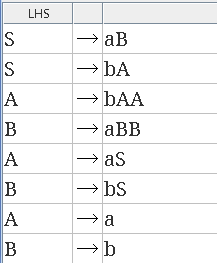
\includegraphics[width=\textwidth]{./Imagenes/image1.png}
                    \caption{la producción}
                    \label{fig:label1}
                \end{subfigure}
                \hfill
                \begin{subfigure}[b]{0.55\textwidth}
                    \centering
                    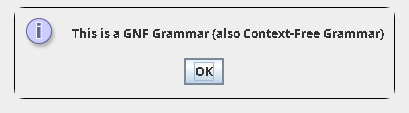
\includegraphics[width=\textwidth]{./Imagenes/image2.png}
                    \caption{gramatica libre contexto}
                    \label{fig:label2}
                \end{subfigure}
                \vspace{0.5cm} 
                \\
                \begin{subfigure}[b]{0.35\textwidth}
                    \centering
                    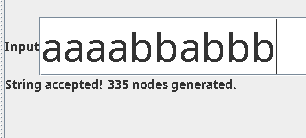
\includegraphics[width=\textwidth]{./Imagenes/image3.png}
                    \caption{cadena $aaaabbabbb$}
                    \label{fig:label3}
                \end{subfigure}
                \label{fig:matrix1}
            \end{figure}

            \begin{figure}[!h]
                \centering
                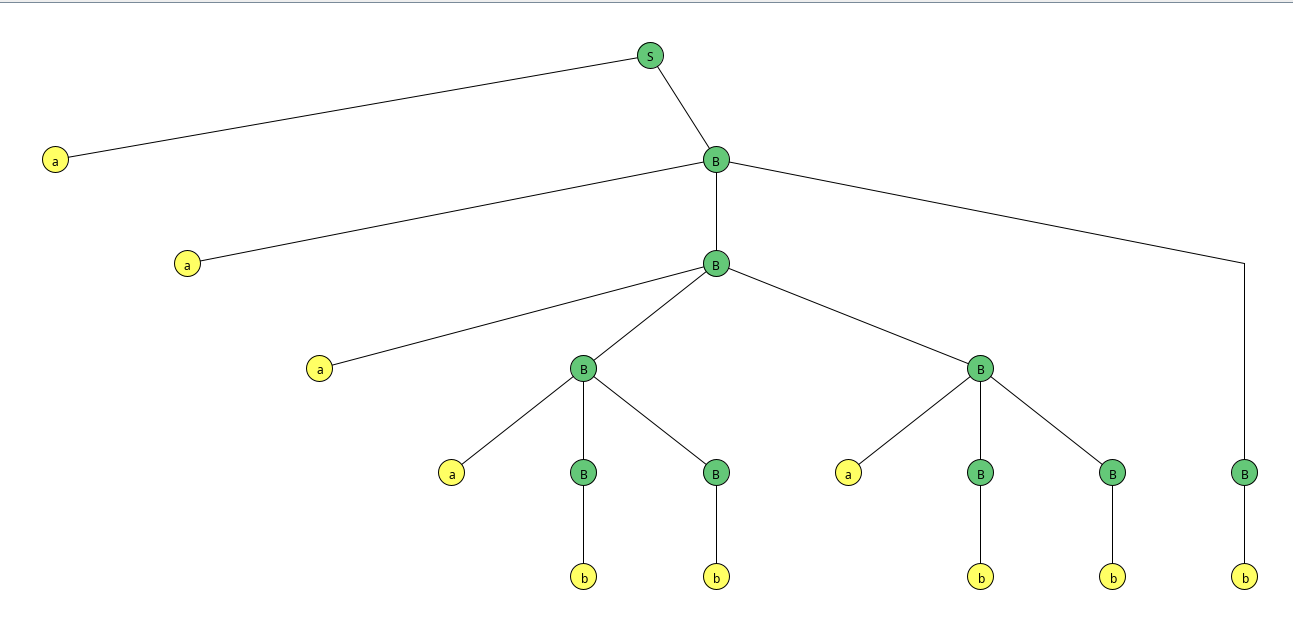
\includegraphics[width=\textwidth]{./Imagenes/image4.png}
                \caption{la cadena $aabb$}
                \label{fig:label4}
            \end{figure}
            
            
            

                
        \newpage




        % 
        % Ejercicio 2
        %

        \section*{Ejercicio 2}
        \begin{enumerate}
            \item \textbf{determina si la gramática $G = (\{S,A,B\}, \{a,b,c,d\}. P,S)$ donde $P$ es el conjunto regla producción
            genera un lenguaje tipo 3.}
            
            \begin{tabularx}{\textwidth}{XXX}
                $S \rightarrow AB$ & $A \rightarrow Ab$ & $A \rightarrow a$\\
                $B \rightarrow cB$ & $B \rightarrow d$\\
            \end{tabularx}
            
            \item \textbf{obtener el ATDM, (automanta deterministico minimal)
            Obtener el modelo de cálculo más optimo para resolver el problema del apartado A}
        \end{enumerate}
        
        \vspace{\baselineskip} % paso linea

        \textbf{Apartado 1:}
        Es un tipico problema de optimizacion. Primero nos fijamos en que no es una gramatica regular por producciones
        como $B \rightarrow cB$ o $A \rightarrow Ab$
        Generar un lenguaje de tipo 3 significa que sea libre de contexto
        Estudio una produccion de ejemplo
        $$ S \rightarrow AB \rightarrow AbB \rightarrow AbbB \rightarrow abbcB \rightarrow abbccB \rightarrow abbcccB \rightarrow abbcccd$$ 

        Si nos fijameos genera el lenguaje $L = \{ab^ic^jd : i, j \in \mathbb{N}  \}$, vemos si existe una gramatica libre de contexto que genere este lenguaje,
        es decir optimizamos.

        \vspace{\baselineskip} % paso linea
        Este lenguaje se genera con la gramatica $G = (\{S,A,B\}, \{a,b,c,d\}. P,S)$ donde $P$ es el conjunto regla producción
        \vspace{\baselineskip} % paso linea

        \begin{tabularx}{\textwidth}{XXX}
            $S \rightarrow AB$ & $B \rightarrow C$ & $C \rightarrow d$\\
            $B \rightarrow bB$ & $C \rightarrow cC$\\
        \end{tabularx}

        \vspace{\baselineskip} % paso linea
        \textbf{Comprobacion con JFLAP}
            \begin{figure}[!h] 
            \centering
                \centering
                \begin{subfigure}[b]{0.35\textwidth}
                    \centering
                    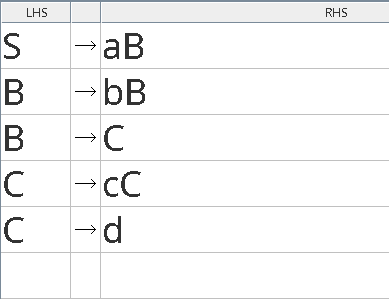
\includegraphics[width=\textwidth]{./Imagenes/image8.png}
                    \caption{la producción}
                    \label{fig:label1}
                \end{subfigure}
                \hfill
                \begin{subfigure}[b]{0.55\textwidth}
                    \centering
                    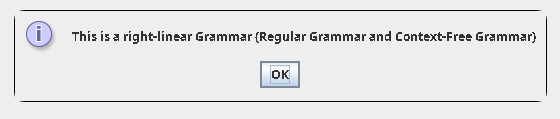
\includegraphics[width=\textwidth]{./Imagenes/image5.png}
                    \caption{gramatica libre contexto}
                    \label{fig:label2}
                \end{subfigure}
                \vspace{0.5cm} 
                \\
                \begin{subfigure}[b]{0.25\textwidth}
                    \centering
                    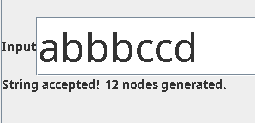
\includegraphics[width=\textwidth]{./Imagenes/image7.png}
                    \caption{cadena $abbbccd$}
                    \label{fig:label3}
                \end{subfigure}
                \label{fig:matrix1}
            \end{figure}


        \newpage


        \begin{figure}[!h]
            \centering
            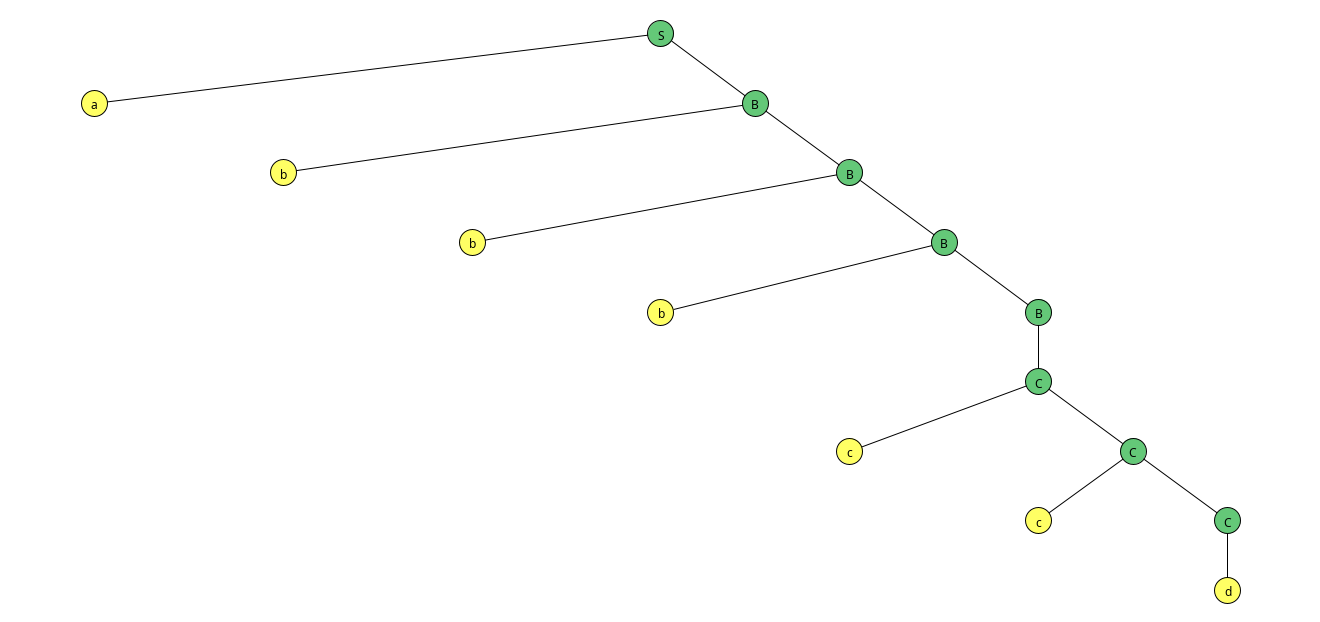
\includegraphics[width=\textwidth]{./Imagenes/image6.png}
            \caption{la cadena $aabb$}
            \label{fig:label4}
        \end{figure}
        \vspace{\baselineskip} % paso linea
        \textbf{Apartado 2:}

        Automata no deterministico con transiciones nulas
        Con la produccion anterior en JFLAP he insertado la gramatica y luego he Convert-right linear gramar to FA
        \vspace{\baselineskip} % paso linea

            \begin{figure}[!h] 
            \centering
                \centering
                \begin{subfigure}[b]{0.55\textwidth}
                    \centering
                    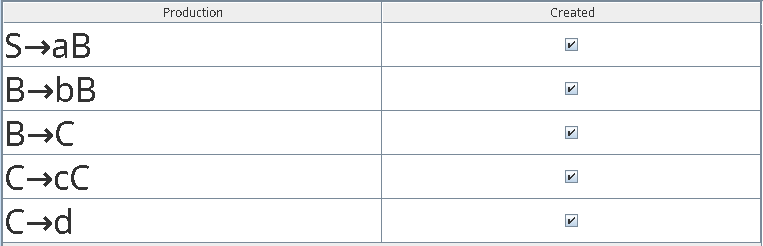
\includegraphics[width=\textwidth]{./Imagenes/image10.png}
                    \label{fig:label1}
                \end{subfigure}
                \hfill
                \begin{subfigure}[b]{1.05\textwidth}
                    \centering
                    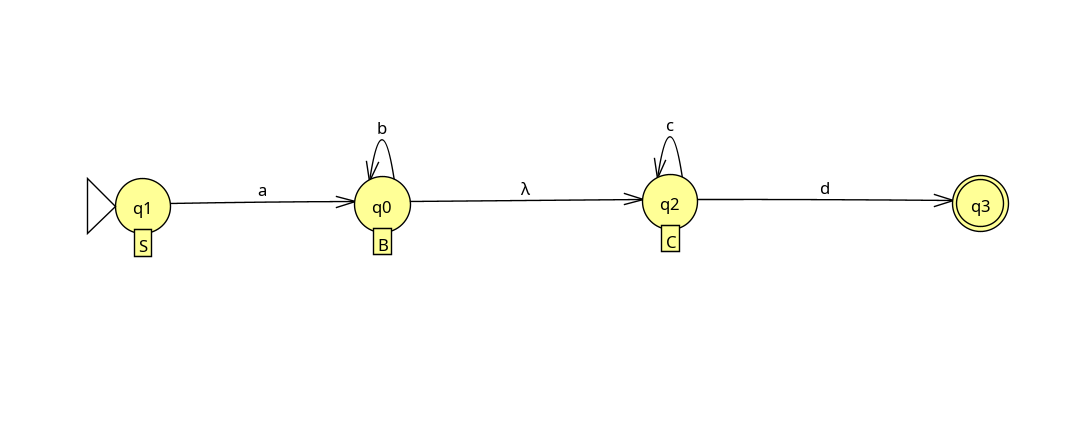
\includegraphics[width=\textwidth]{./Imagenes/image9.png}
                    \label{fig:label2}
                \end{subfigure}
                \vspace{0.5cm} 
            \end{figure}
        
        Automata finito deterministico
        Con un FA, le doy a convert to DFA (automata finito deterministico)
        \begin{figure}[!h]
            \centering
            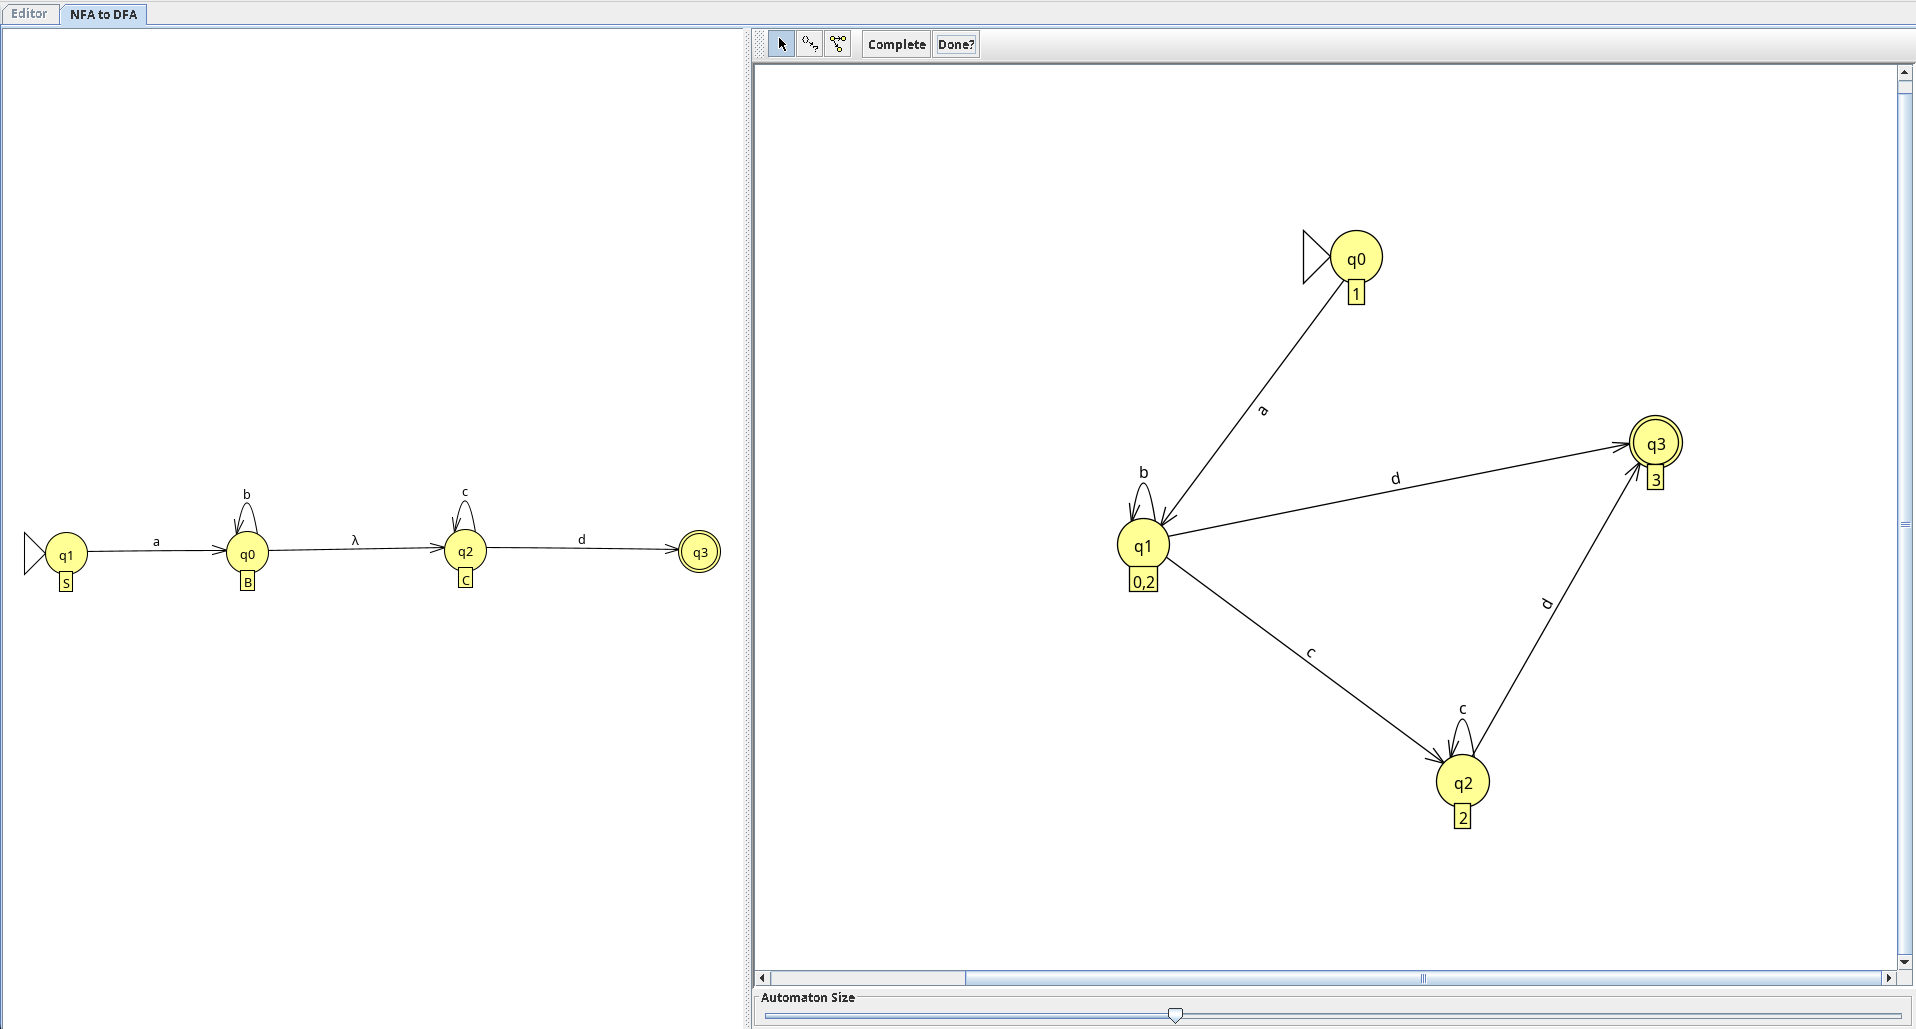
\includegraphics[width=1.2\textwidth]{./Imagenes/image11.png}
            \label{fig:label4}
        \end{figure}

        Automata finito deterministico minimal
        desde el DFA en convert a minimize DFA, vemos que no se puede minimizar por que da el anterior
        \begin{figure}[!h]
            \centering
            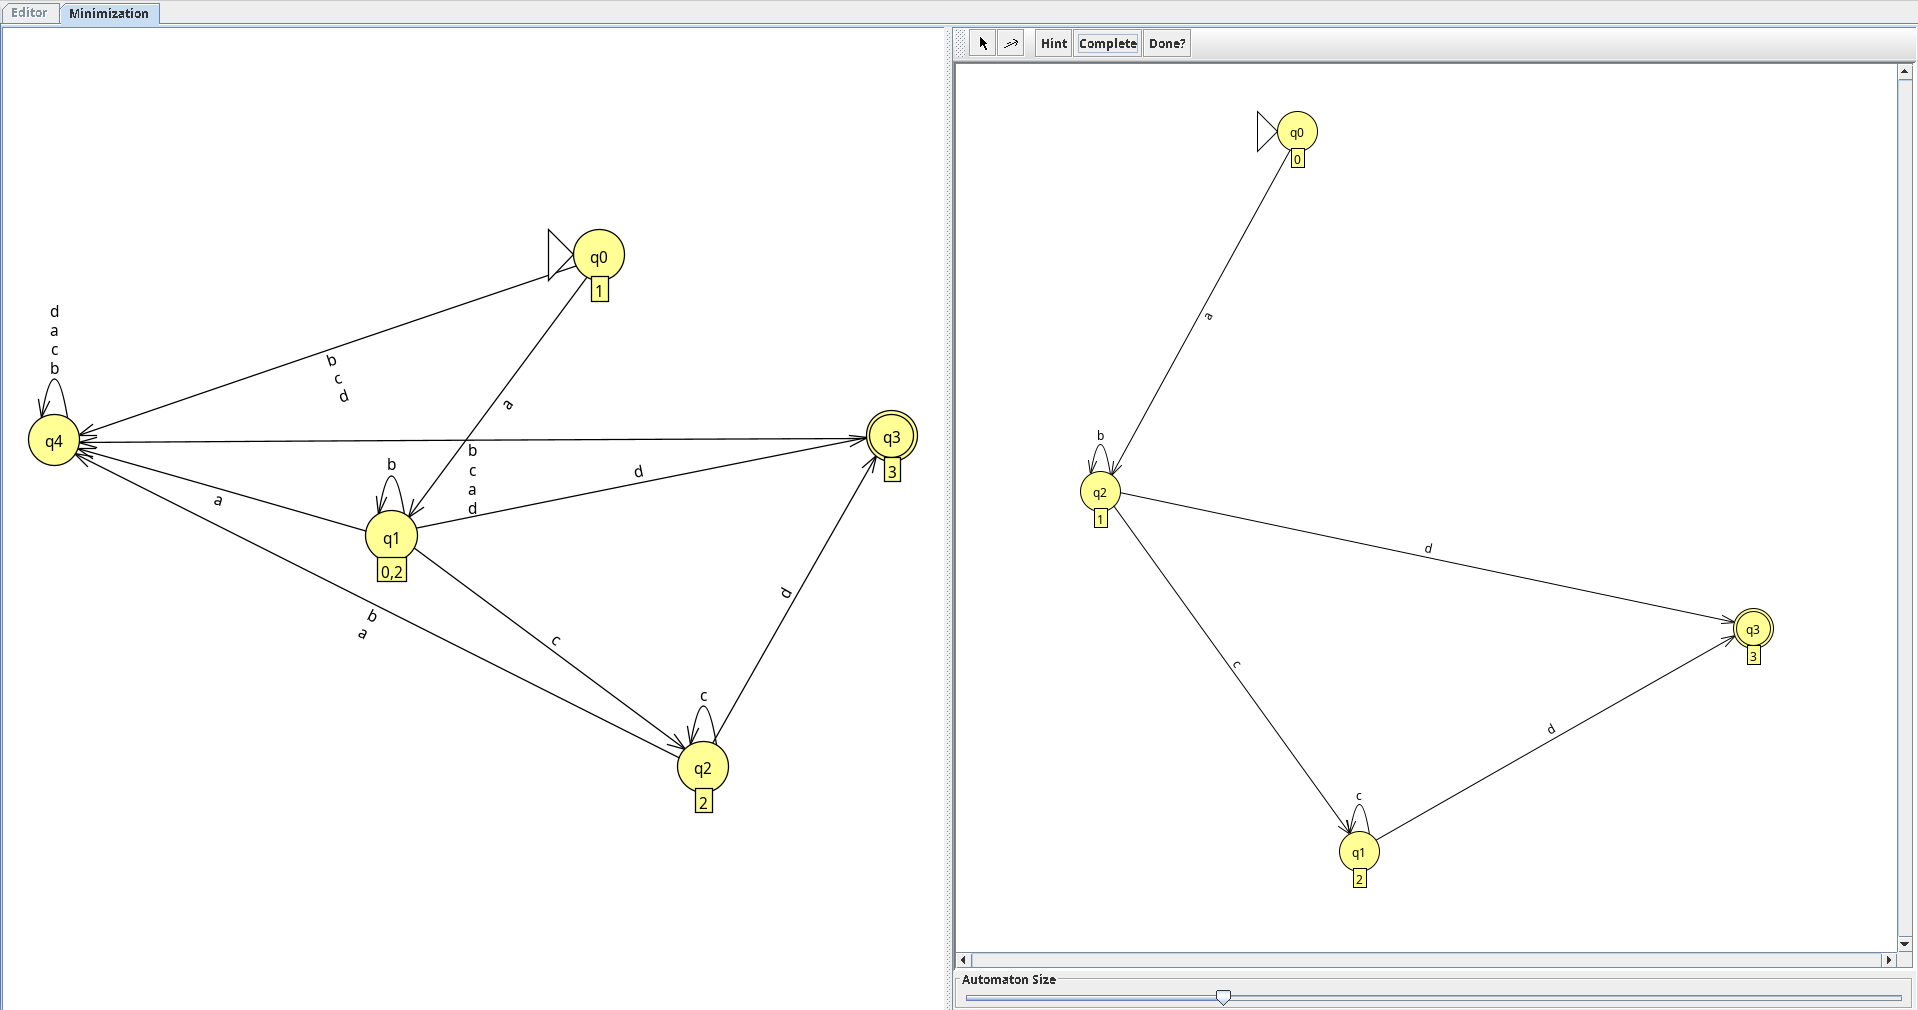
\includegraphics[width=1.2\textwidth]{./Imagenes/image12.png}
            \label{fig:label4}
        \end{figure}


        Ejemplo de ejecucion
        \begin{figure}[!h]
            \centering
            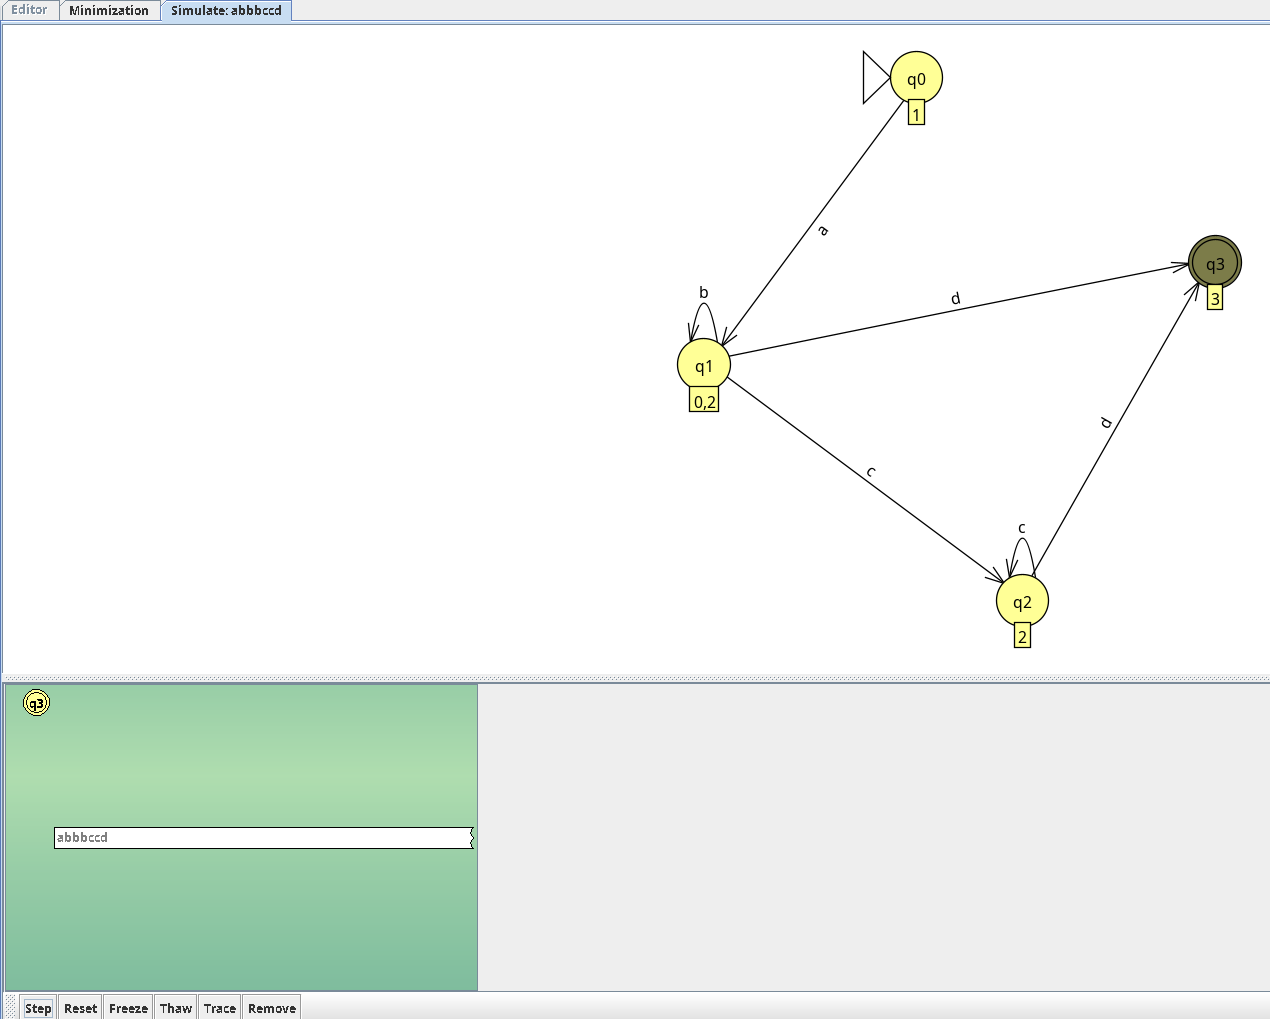
\includegraphics[width=1.2\textwidth]{./Imagenes/image13.png}
            \label{fig:label4}
        \end{figure}



            

        \newpage

        % 
        % Ejercicio 3
        %
        \section*{Ejercicio 3}
        \textbf{Apartado 1: construir una expresión regular para las palabras en las que numeros de ceros es par}
        
        \vspace{\baselineskip} % paso linea

        $$ 1*(01*01*)*$$
        Forzamos a de esta manera que comience por 1 y que vayan apareciendo ceros de manera par , de dos en dos
        
        Regular expresion to NFA
        NFA a DFA (deterministico)
       
        \begin{figure}[!h]
            \centering
            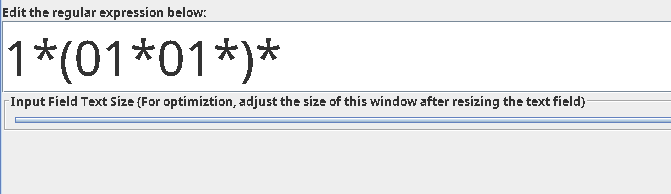
\includegraphics[width=0.4\textwidth]{./Imagenes/image19.png}
            \label{fig:label4}
            \caption{Expresion regular}
        \end{figure}

        \begin{figure}[!h]
            \centering
            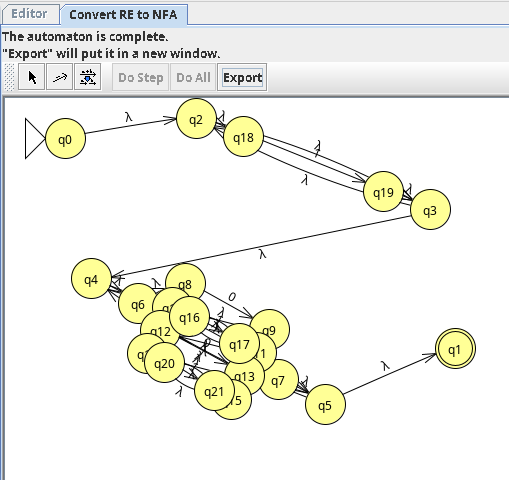
\includegraphics[width=0.8\textwidth]{./Imagenes/image14.png}
            \label{fig:label4}
            \caption{Automata finito no deterministico}
        \end{figure}

        \newpage

        \begin{figure}[!h]
            \centering
            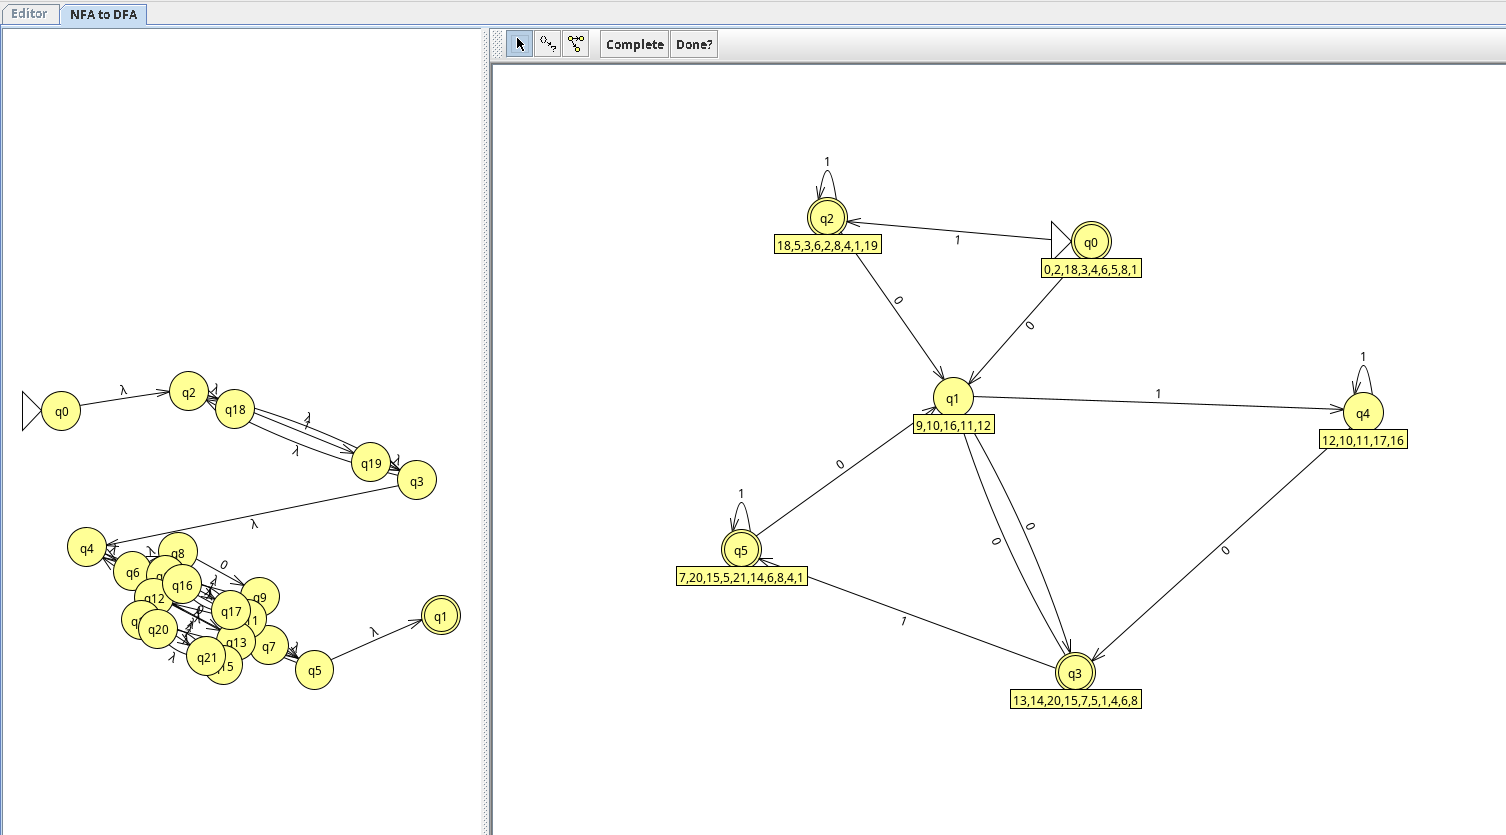
\includegraphics[width=1.2\textwidth]{./Imagenes/image15.png}
            \label{fig:label4}
            \caption{Automata finito  deterministico}
        \end{figure}

        \begin{figure}[!h]
            \centering
            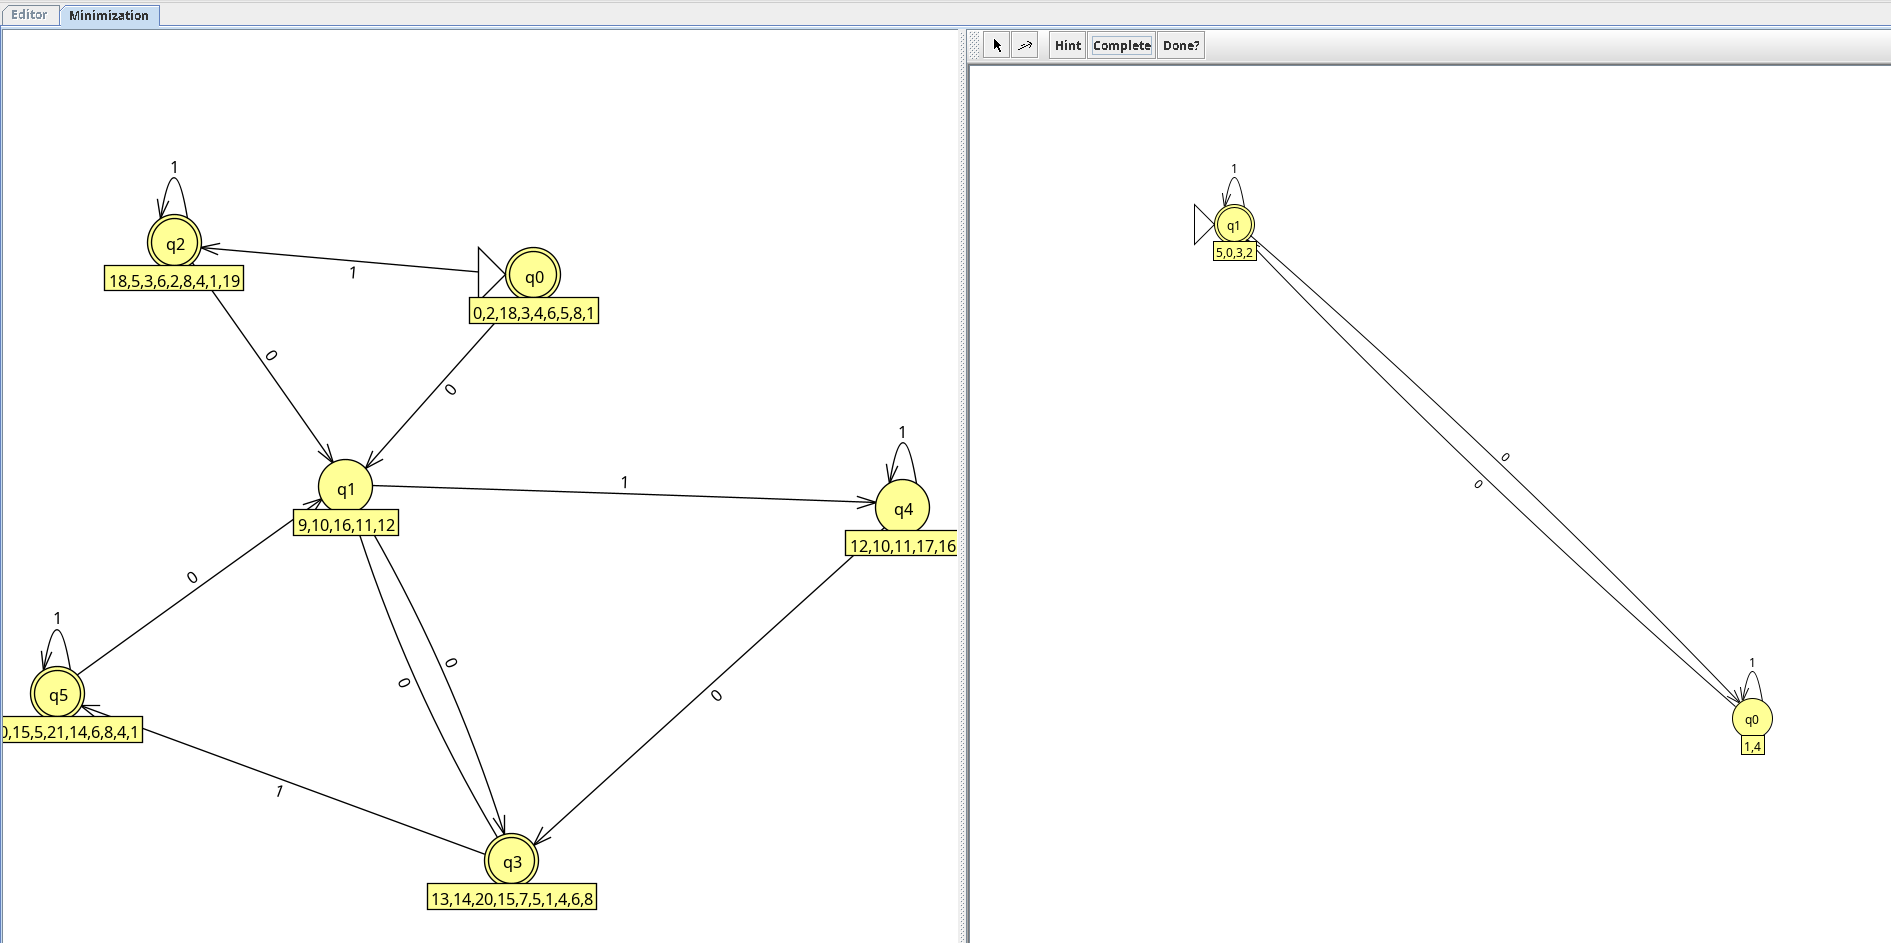
\includegraphics[width=1.2\textwidth]{./Imagenes/image16.png}
            \label{fig:label4}
            \caption{Automata finito deterministico minimal}
        \end{figure}

        \newpage
        \begin{figure}[!h]
            \centering
            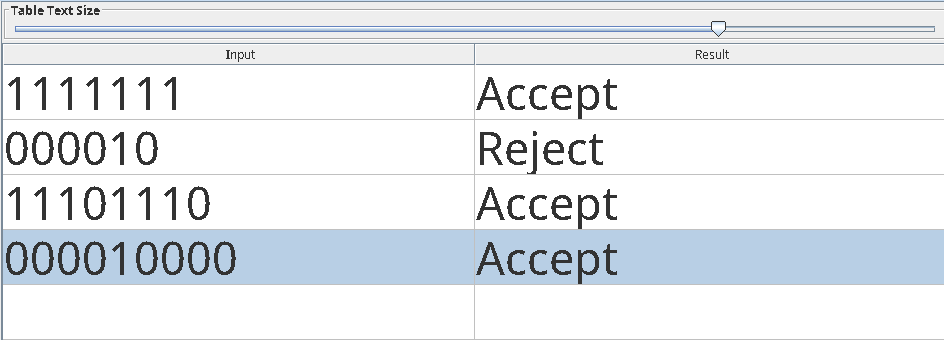
\includegraphics[width=0.8\textwidth]{./Imagenes/image17.png}
            \label{fig:label4}
            \caption{ejemplo de ejecucion}
        \end{figure}

        \vspace{\baselineskip} % paso linea
        \textbf{Apartado 2: Construir una expresion regular para las palabras que contengan a 01100 como subcadena }
         $$(0+1)*0110(0+1)*$$
        Una cadena que comience y termine por cualquier combinacion de 0 y 1 y contenga 0110

        \begin{figure}[!h]
            \centering
            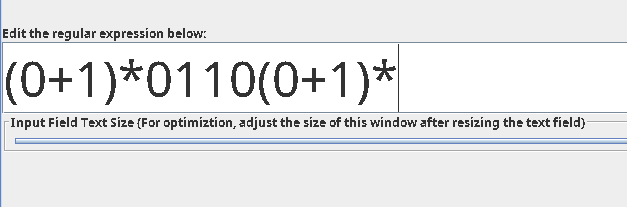
\includegraphics[width=0.4\textwidth]{./Imagenes/image25.png}
            \label{fig:label4}
            \caption{Expresion regular}
        \end{figure}

        \begin{figure}[!h]
            \centering
            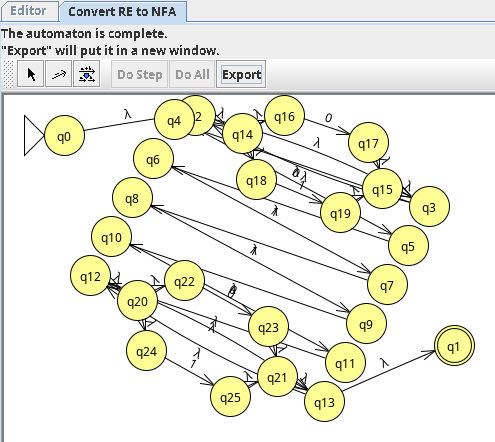
\includegraphics[width=0.55\textwidth]{./Imagenes/image26.png}
            \label{fig:label4}
            \caption{Automata finito no deterministico}
        \end{figure}

        \newpage

        \begin{figure}[!h]
            \centering
            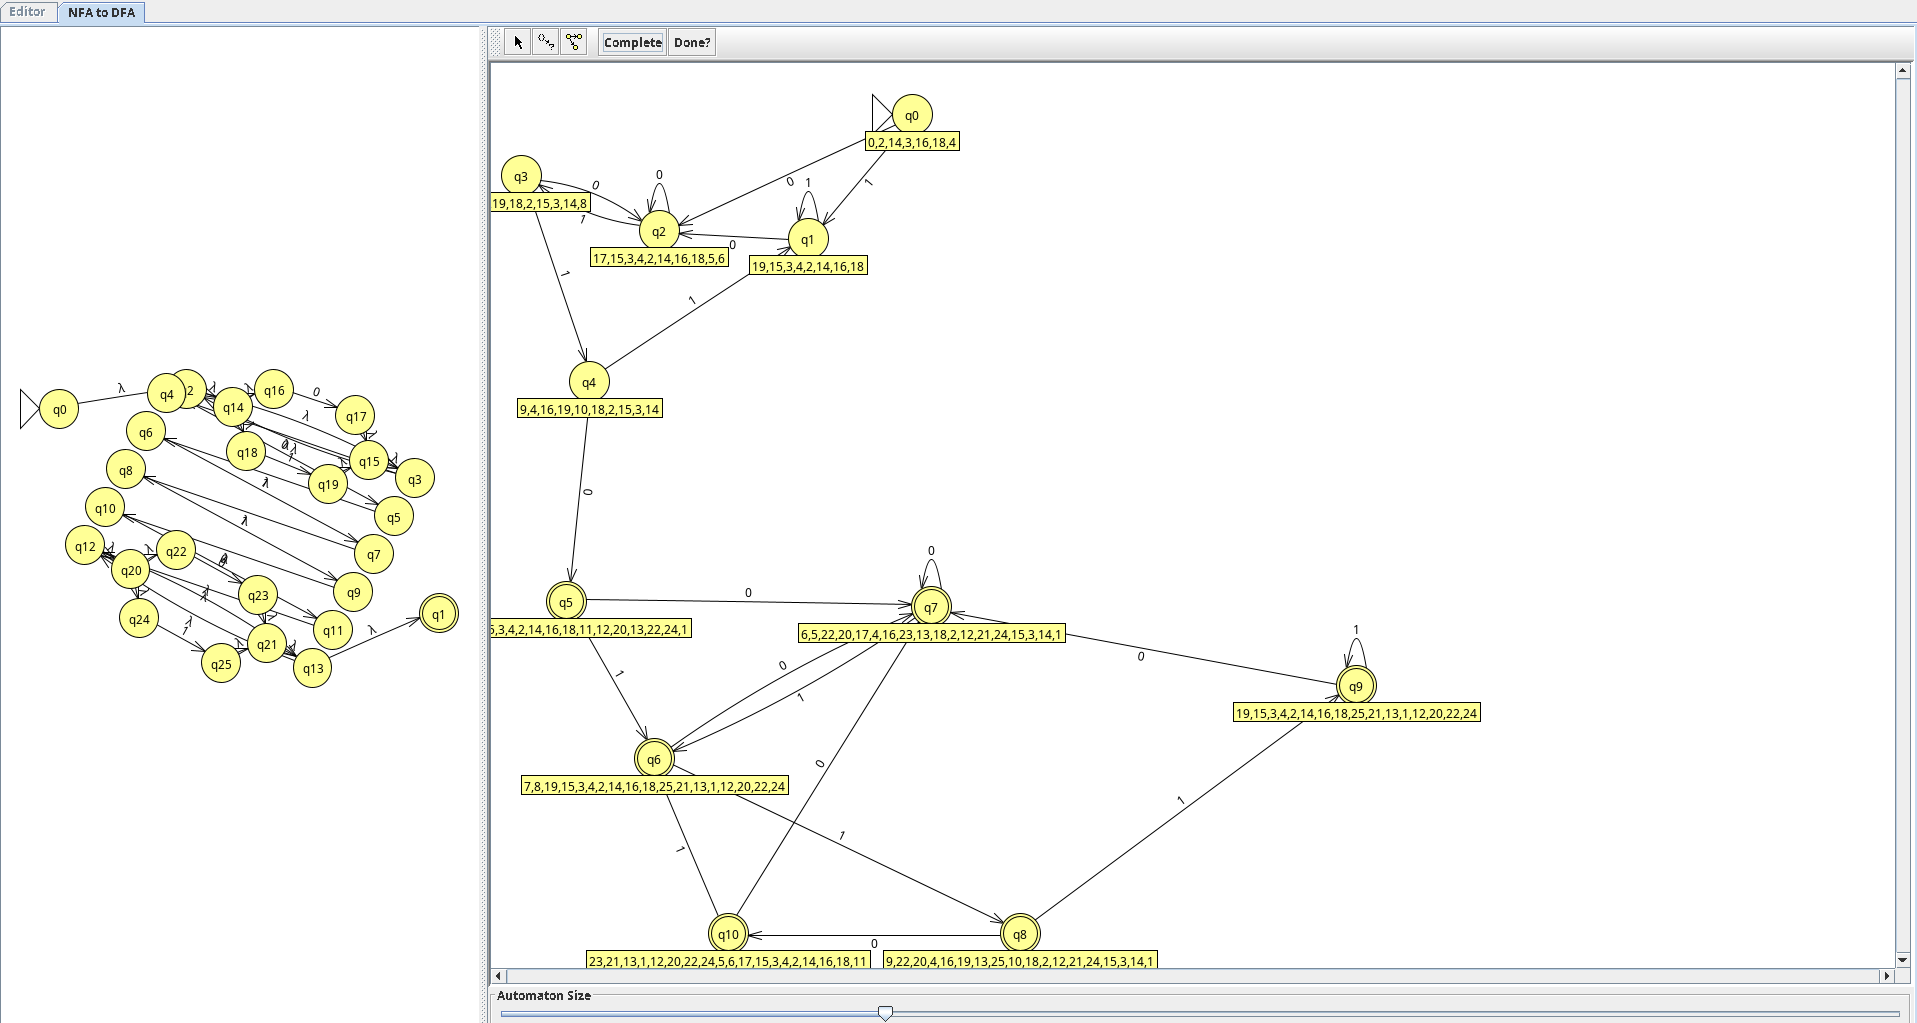
\includegraphics[width=1.2\textwidth]{./Imagenes/image27.png}
            \label{fig:label4}
            \caption{Automata finito  deterministico}
        \end{figure}

        \begin{figure}[!h]
            \centering
            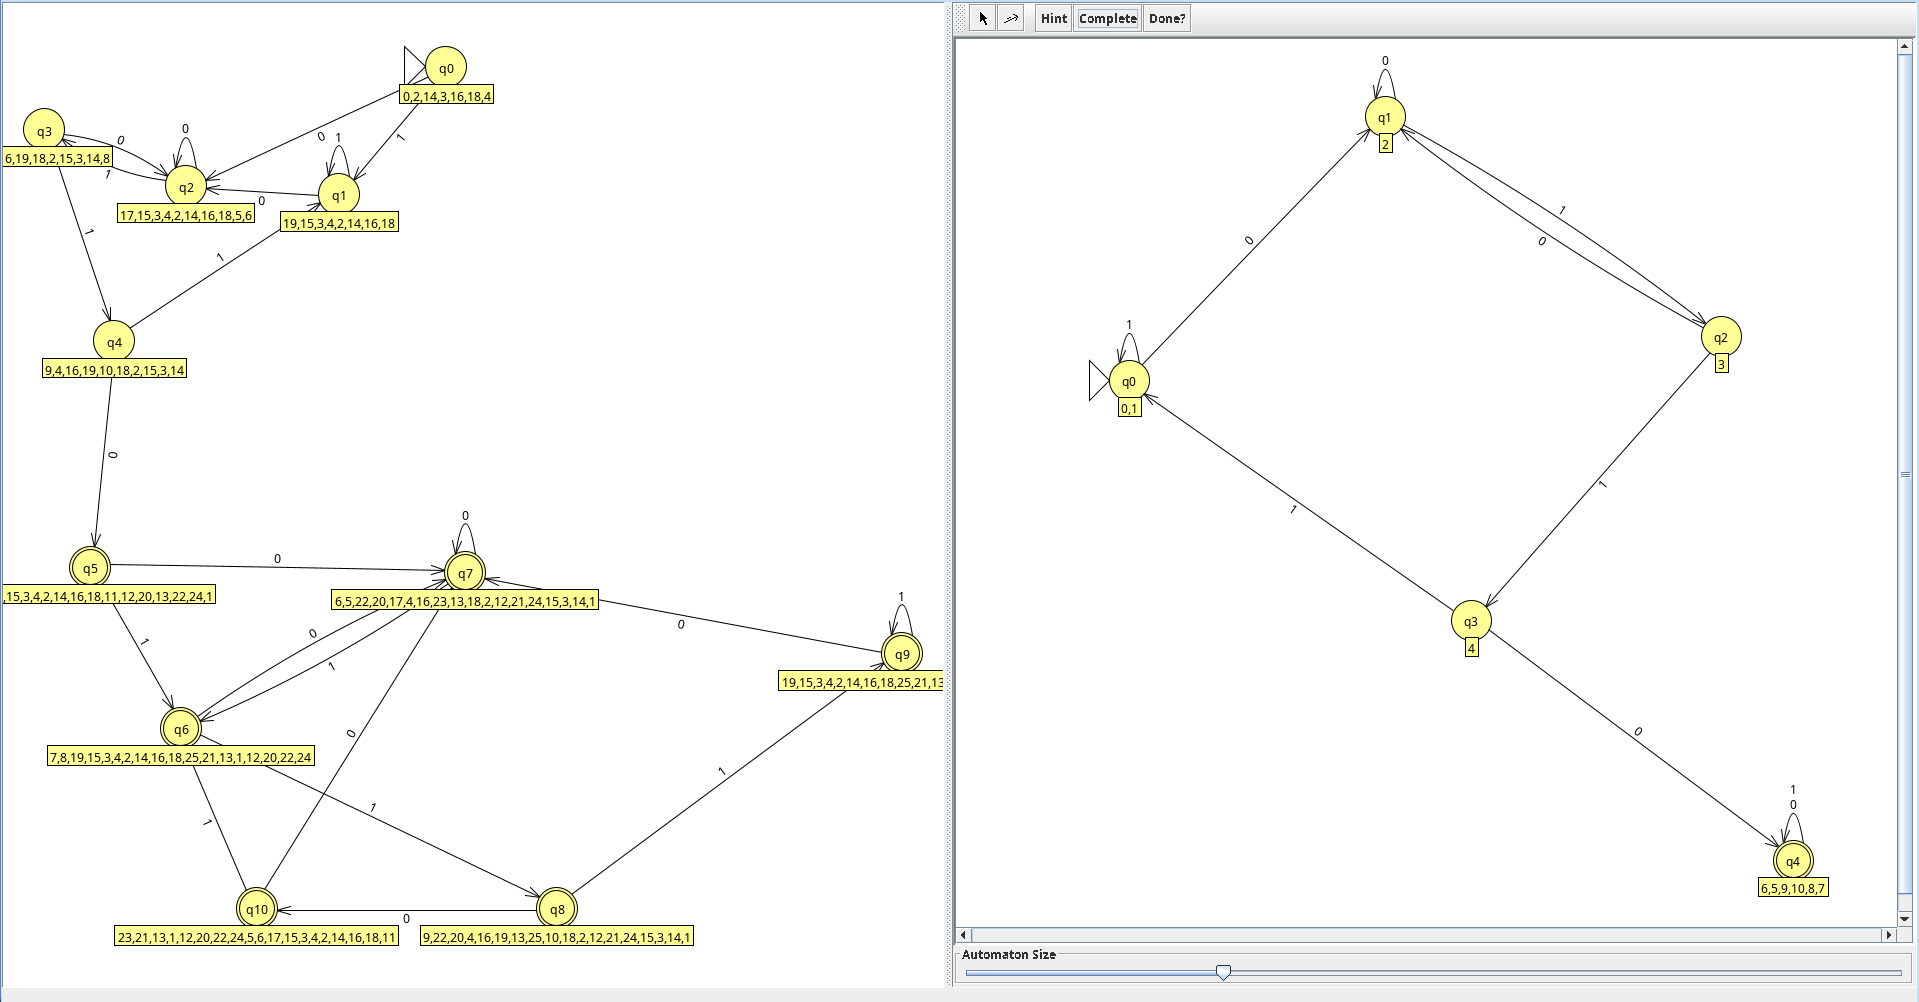
\includegraphics[width=1.2\textwidth]{./Imagenes/image28.png}
            \label{fig:label4}
            \caption{Automata finito deterministico minimal}
        \end{figure}

        \newpage
        \begin{figure}[!h]
            \centering
            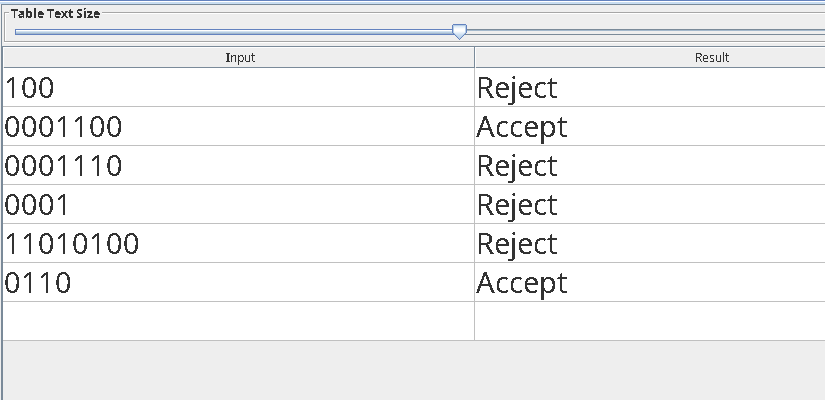
\includegraphics[width=0.8\textwidth]{./Imagenes/image29.png}
            \label{fig:label4}
            \caption{ejemplo de ejecucion}
        \end{figure}

        \textbf{Apartado 3: Construir una expresion regular para el conjunto de palabras que empiezan por 000 y tales que esta subcadena solo se encuentra al principio de la palabra}
        $$ 000(1+10+100)*$$
        Comienza por 000 y luego no vuelve a aparecer 000
        
        \begin{figure}[!h]
            \centering
            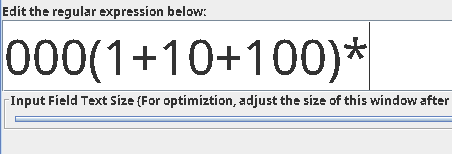
\includegraphics[width=0.4\textwidth]{./Imagenes/image20.png}
            \label{fig:label4}
            \caption{Expresion regular}
        \end{figure}

        \begin{figure}[!h]
            \centering
            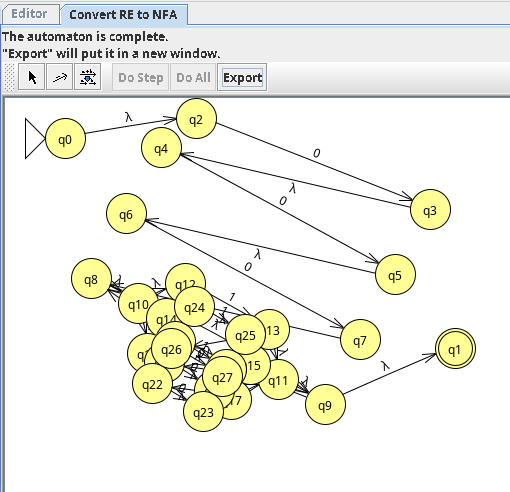
\includegraphics[width=0.5\textwidth]{./Imagenes/image21.png}
            \label{fig:label4}
            \caption{Automata finito no deterministico}
        \end{figure}

        \newpage

        \begin{figure}[!h]
            \centering
            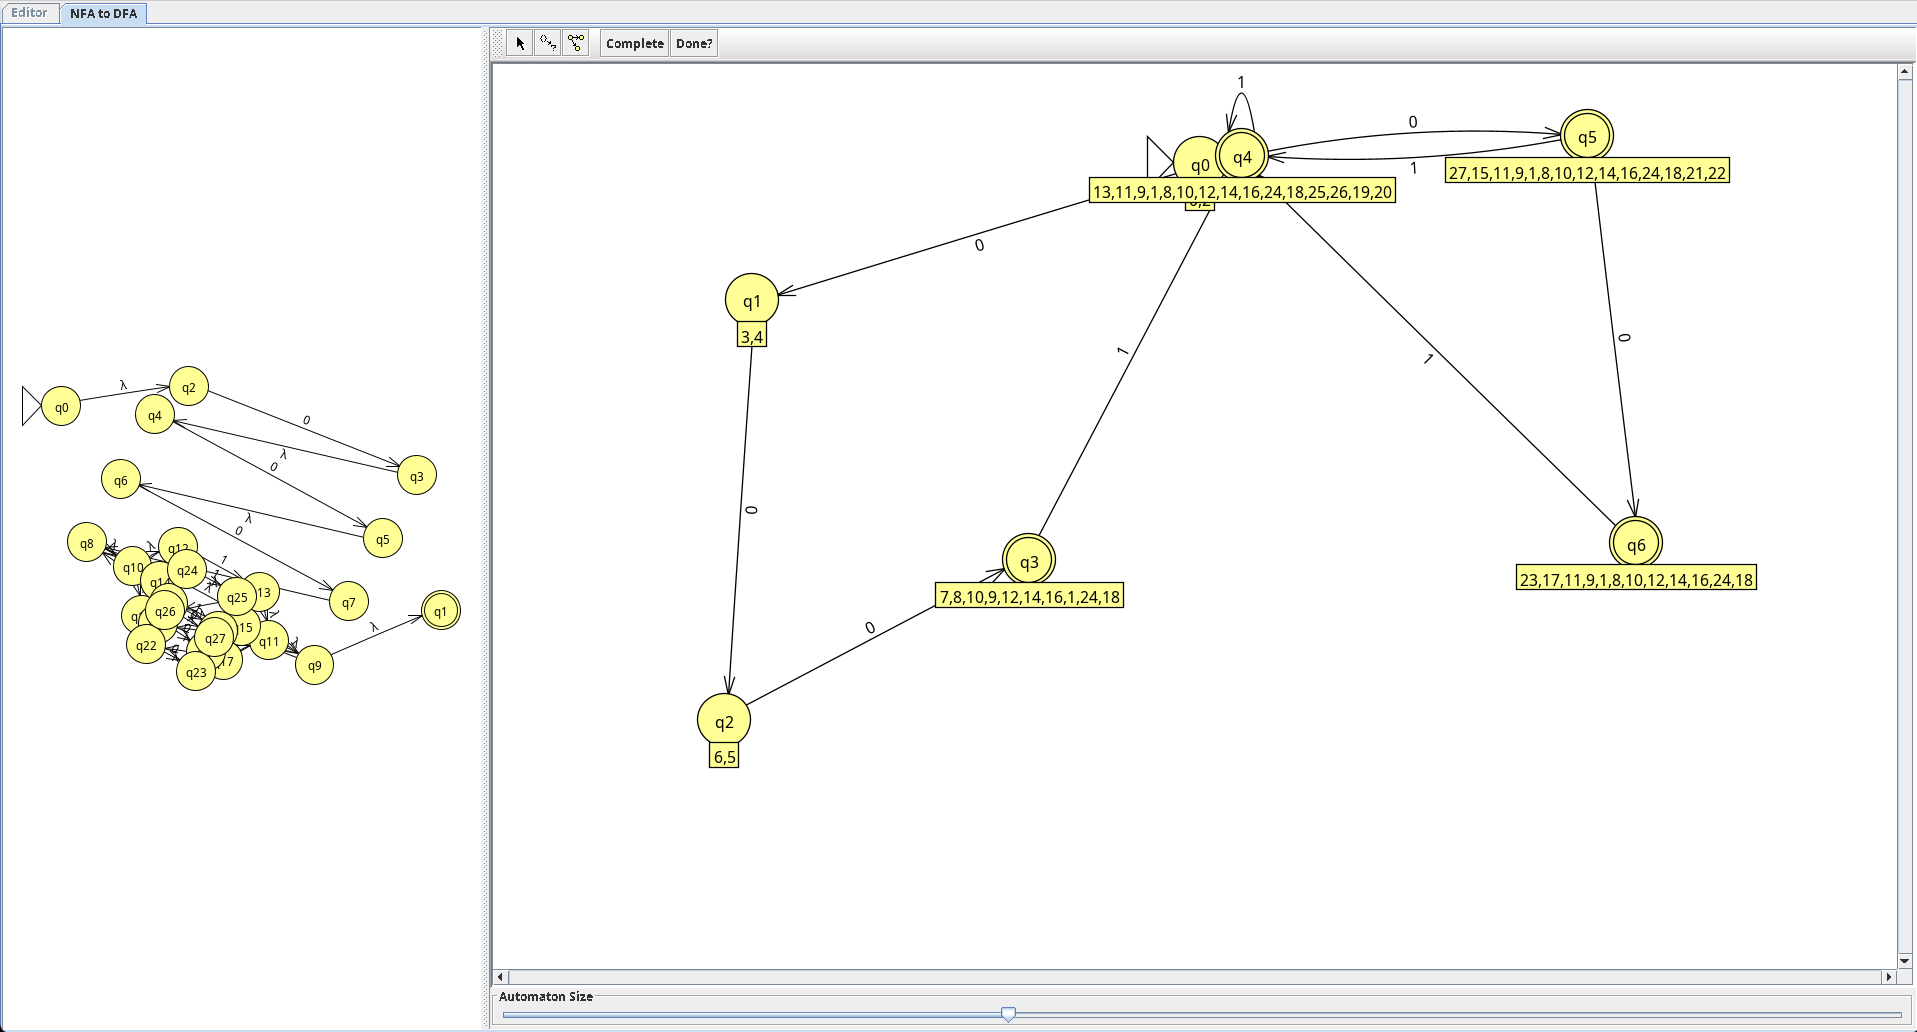
\includegraphics[width=1.2\textwidth]{./Imagenes/image22.png}
            \label{fig:label4}
            \caption{Automata finito  deterministico}
        \end{figure}

        \begin{figure}[!h]
            \centering
            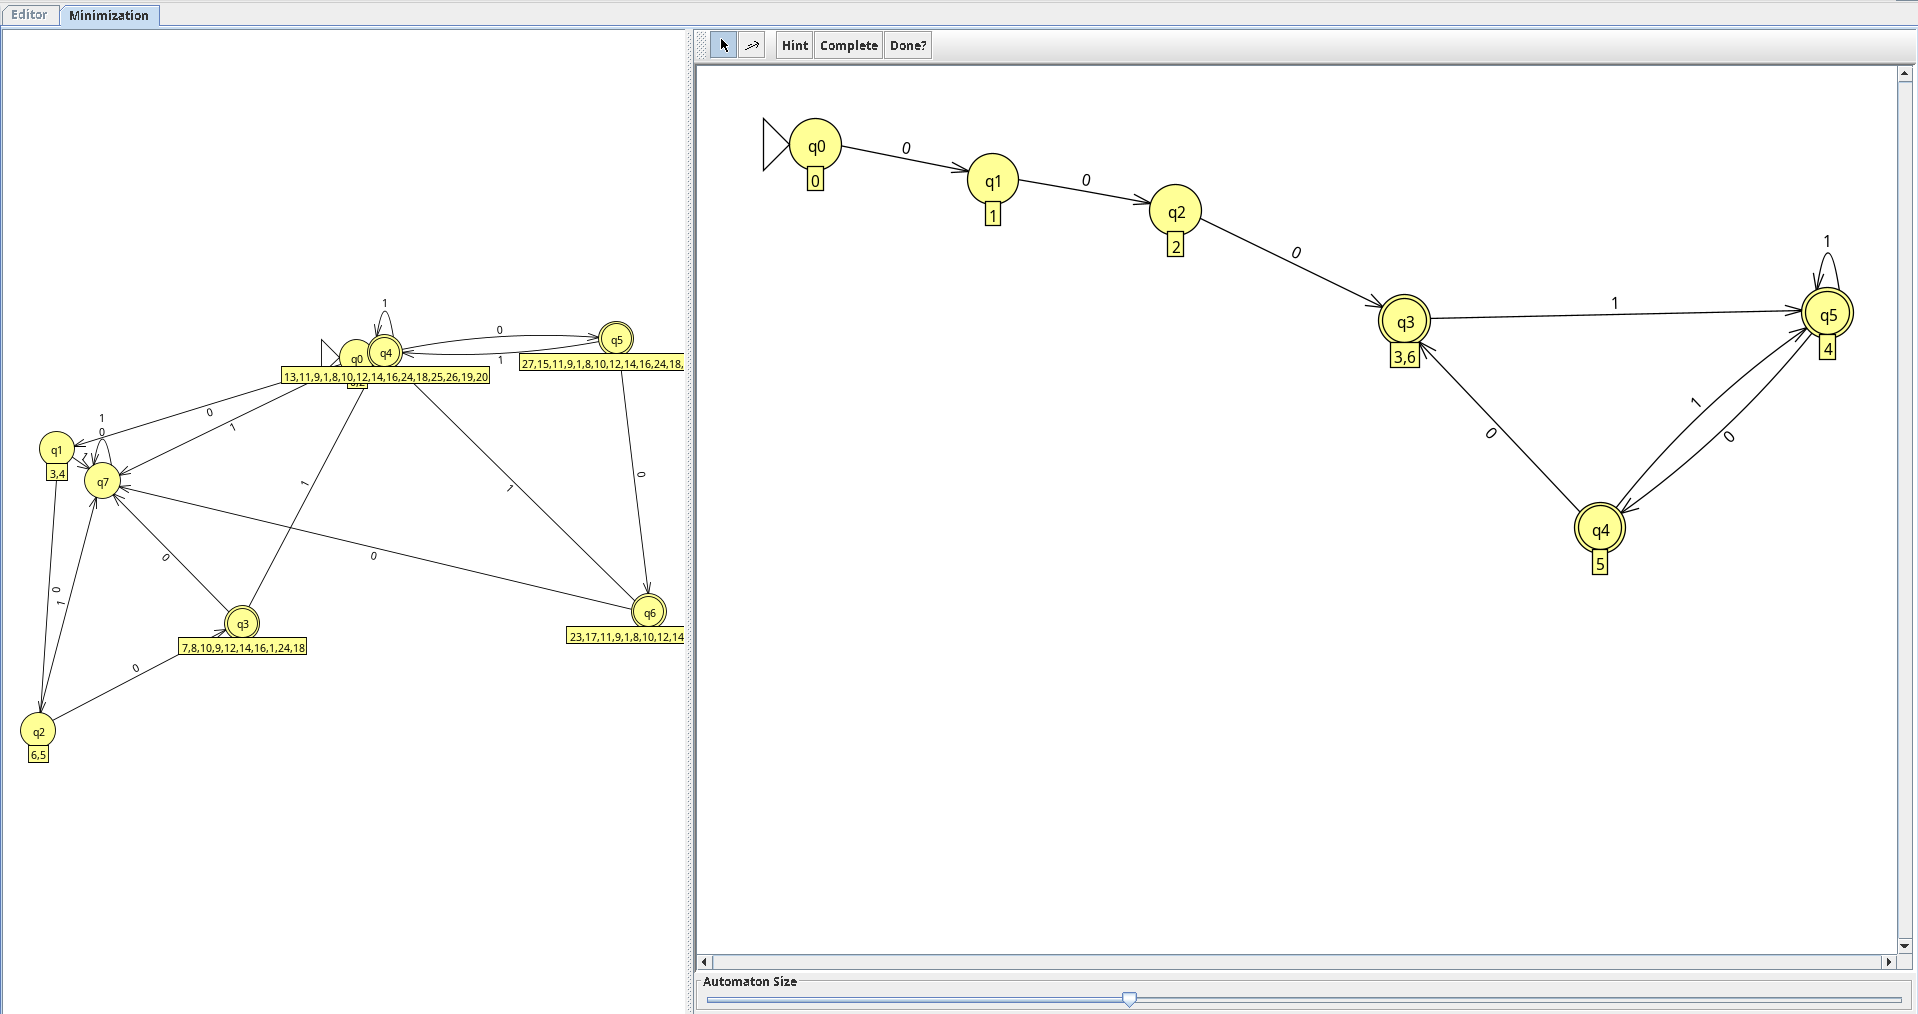
\includegraphics[width=1.2\textwidth]{./Imagenes/image23.png}
            \label{fig:label4}
            \caption{Automata finito deterministico minimal}
        \end{figure}

        \newpage
        \begin{figure}[!h]
            \centering
            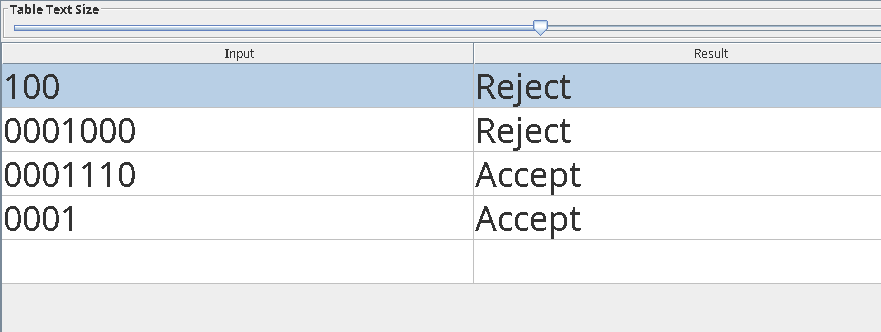
\includegraphics[width=0.8\textwidth]{./Imagenes/image24.png}
            \label{fig:label4}
            \caption{ejemplo de ejecucion}
        \end{figure}

        


        \newpage

        % 
        % Ejercicio 4
        %

        \section*{Ejercicio 4}
        \begin{enumerate}
            \item \textbf{¿Es $L = \{ U \in \{0, 1\}^* /\  u=u^{-1} \}$. regular? }
            \item \textbf{Encontrar un modelo de calculo para $L$ }
        \end{enumerate}

        Definimos el Lema de Bombeo: Sea \( L \) un conjunto regular. Entonces, existe un \( n \in \mathbb{N} \) tal que para todo \( z \in L \) con \( |z| \geq n \), se puede expresar como \( z = u v w \) donde:
        \begin{enumerate}
          \item \( |uv| \leq n \)
          \item \( |v| \geq 1 \)
          \item Para todo \( i \in \mathbb{N} \), \( uv^iw \in L \)
        \end{enumerate}
        Además, el número de estados de cualquier autómata que acepta el lenguaje \( L \) es al menos \( n \).
        \vspace{\baselineskip} % Salto de línea

        La idea básica del lema de bombeo es que para cualquier cadena lo suficientemente larga, 
        puedes "bombear" o repetir una parte de la cadena y 
        aún obtener una cadena en el lenguaje. 
        Este lema siempre es verdadero para lenguajes regulares. 
        Si no es verdadero para un lenguaje, entonces ese lenguaje 
        no es regular. Para demostrar esto, buscamos un contraejemplo.
        
        \vspace{\baselineskip} % Salto de línea
        
        
        Suponemos lo contrario: \( L \) es regular y satisface el lema de bombeo. Buscamos un contraejemplo.
        \[ \exists n \in \mathbb{N},\quad \forall Z \in L,\quad |Z| \geq n,\quad Z = 0^n 1^n 0^n = uvw \]
        
        
        Aplicamos \( |uv| \leq n \):
        \[ uv = 0^k, \quad v = 0^l, \quad w = 0^{n-k-l}1^n0^n \]
        
        \( |v| \geq 1 \) implica que \( v = 0^l \) y \( l \geq 1 \).
        \vspace{\baselineskip} % Salto de línea

        Para \( i \geq 2 \), verificamos \( uv^iw \in L \):
        \[ i = 2\quad  uv^2w = 0^k 0^{2l} 0^{n-k-l} 1^n 0^n =\quad 0^{n+l} 1^n 0^n \notin L \]
           
        Hemos alcanzado una contradicción con el lema de bombeo, por lo que \( L \) no es regular.
        
        \vspace{\baselineskip} % paso linea

        
        \newpage
        \textbf{Apartado 2: Obtener un modelo de calculo para $L$}         \vspace{\baselineskip} % paso linea

         El modelo es no deterministico, lo que significa que no diferencia cuando cambia entre estados. 
         Simula todos los posibles casos.
         q0 se encarga de la parte de la derecha del palindromo y q1 de la parte izquierda 
         Cuando el numero es par el cambio se hace con el 0 o 1. Cuando el numero es impar el cambio se haria con $\lambda$ 
         
        \begin{figure}[!h]
            \centering
            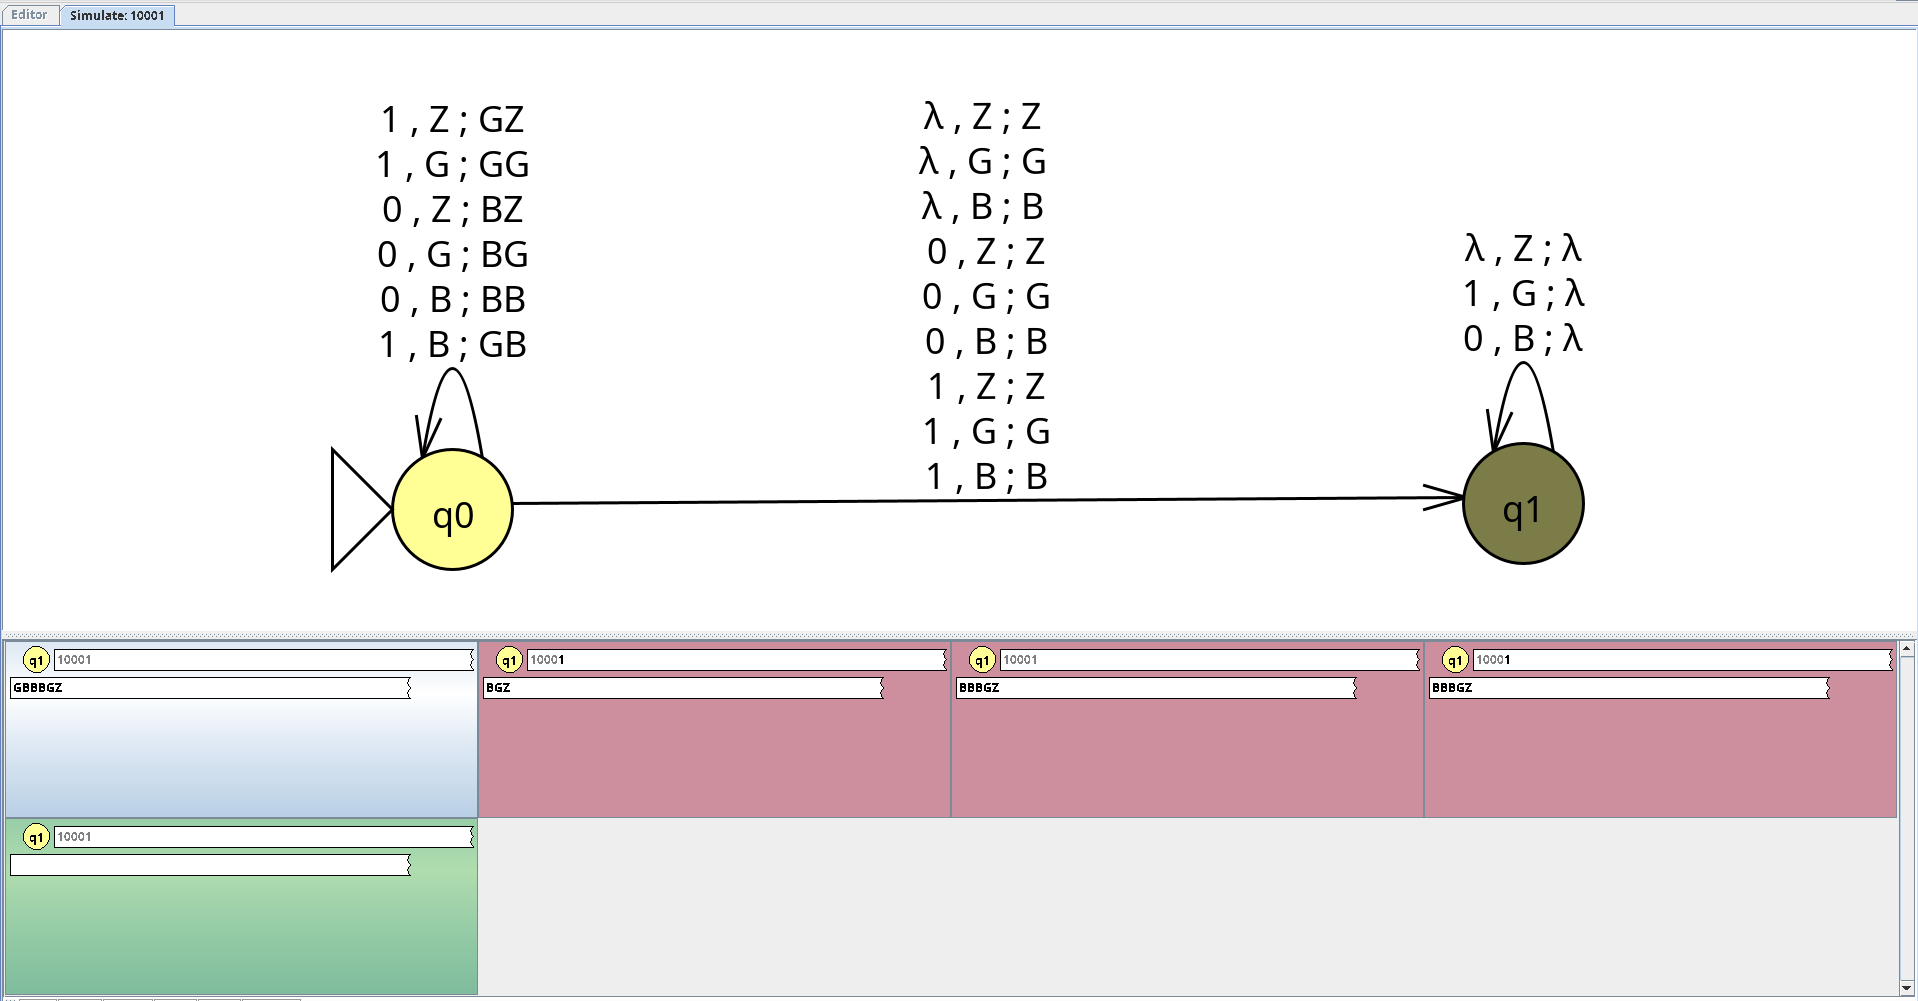
\includegraphics[width=\textwidth]{./Imagenes/image30.png}  
            \label{fig:label4}
            \caption{caso impar 10001}
        \end{figure}

        \begin{figure}[!h]
            \centering
            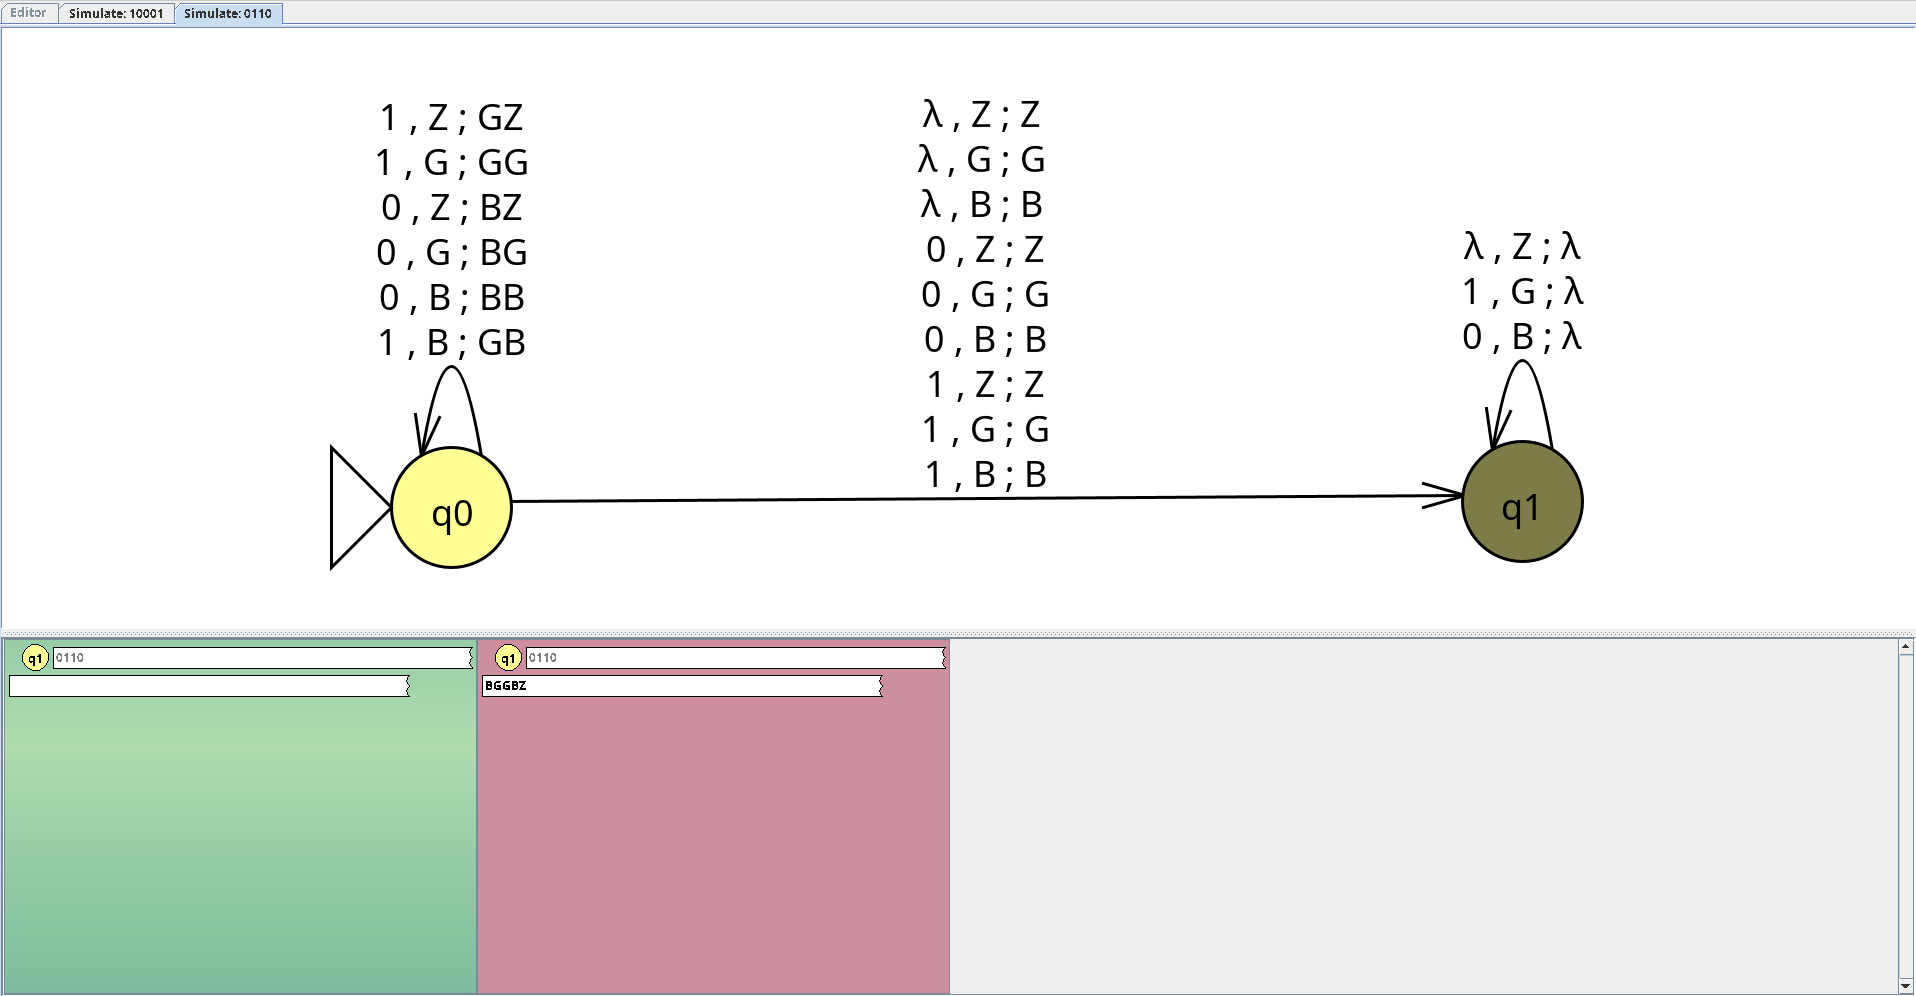
\includegraphics[width=\textwidth]{./Imagenes/image31.png}
            \label{fig:label4}
            \caption{caso par 0110}
        \end{figure}
    \end{document}
